\section*{Introdução}

Pense nas ondas que se produzem quando uma pedra cai na água, ou em como se movimentam as ondas. Pense em como a eletricidade viaja através dos cabos (os quais têm forma de catenária quando se penduram, como sabe bem por artigos anteriores) e pense em como o som se transmite pelo ar até que chega ao seu ouvido. Mais ainda, pense em como a luz chega aos seus olhos e em como os sinais viajam ricocheteando entre satélites.

Pode ser que ainda não o saiba, mas em todos esses casos aparecem as funções periódicas, as quais são tratadas sob um quadro que se conhece como \textit{Análise de Fourier}. Ao longo deste artigo e outros subsequentes vamos conhecer distintos aspetos desta teoria, e se tudo correr bem, chegaremos a um ponto em que poderemos apreciar a enorme influência que exerce nas nossas vidas.

Neste primeiro artigo veremos a parte mais teórica que vamos utilizar em posteriores artigos com aplicações em circuitos elétricos. O artigo presente está dividido como se segue: na secção \ref{s:s1} vamos estudar o que são as funções periódicas e o que são os harmónicos; na secção \ref{s:s2} vamos dar o teorema de representação de uma função como soma de harmónicos na sua versão real e na secção \ref{s:s3} faremos o mesmo, mas da perspetiva do campo complexo, o qual reduz a teoria e permite uma formulação mais simples.


\section{Preliminares}\label{s:s1}
\subsection{Funções periódicas}
A ideia é intuitiva, mas necessitamos uma definição rigorosa a que cingir-nos.
\begin{mybox}
\textbf{Definição.} Consideremos uma função $f:\mathbb{R}\longrightarrow\mathbb{R}$. Dizemos que $f$ é \textbf{periódica} se existir algum número $T>0$ tal que:
\begin{equation} \label{eq:FuncionPeriodica}
f(x+T) = f(x) \qquad \forall x\in\mathbb{R} .
\end{equation}
Assim, diremos que $T$ é um \textbf{período} de $f$. Entre todos eles, o menor recebe o nome de \textbf{período fundamental}.
\end{mybox}

Este conceito pode ser visualizado muito facilmente, uma vez que a equação \eqref{eq:FuncionPeriodica} significa que a gráfica se vai repetindo em intervalos de longitude $T$, como se vê na Figura \ref{fig:FuncionPeriodica}.

\begin{figure}[h]
\begin{figurebox}
    \vspace{5pt}
    \centering
    \scalebox{0.4}{ % Title: glps_renderer figure
% Creator: GL2PS 1.3.8, (C) 1999-2012 C. Geuzaine
% For: Octave
% CreationDate: Mon Aug 11 13:59:37 2014
\setlength{\unitlength}{1pt}
\begin{picture}(0,0)
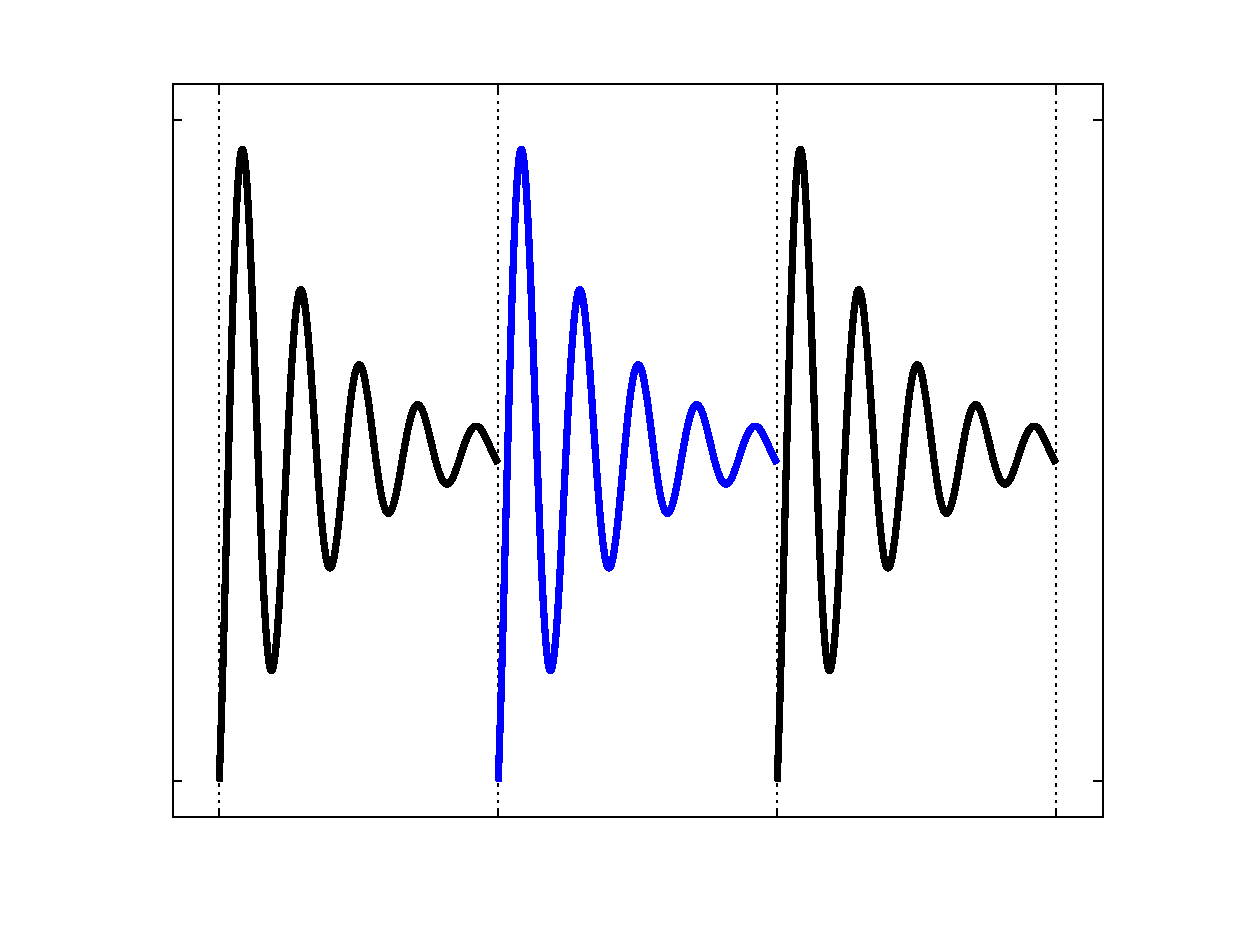
\includegraphics{FuncionPeriodica-inc}
\end{picture}%
\begin{picture}(576,432)(0,0)
\fontsize{30}{0}
\selectfont\put(97.2002,42.519){\makebox(0,0)[t]{\textcolor[rgb]{0,0,0}{{-$T$}}}}
\fontsize{30}{0}
\selectfont\put(231.12,42.519){\makebox(0,0)[t]{\textcolor[rgb]{0,0,0}{{0}}}}
\fontsize{30}{0}
\selectfont\put(365.04,42.519){\makebox(0,0)[t]{\textcolor[rgb]{0,0,0}{{T}}}}
\fontsize{30}{0}
\selectfont\put(498.96,42.519){\makebox(0,0)[t]{\textcolor[rgb]{0,0,0}{{2$T$}}}}
\end{picture}
}
    \vspace{-10pt}
    \caption{Uma função periódica}
    \label{fig:FuncionPeriodica}
\end{figurebox}
\end{figure}

É claro que se $T$ é um período, então $2T$ é um outro período, uma vez que:
\[
f(x+2T) = f((x+T)+T) = f(x+T) = f(x)\qquad \forall x\in \mathbb{R},
\]
e se repetimos o argumento, é fácil ver que
\begin{equation}
  \label{eq:MultiploPeriodo}
  f(x+nT) = f(x) \qquad \forall x\in\mathbb{R},\quad n\in\mathbb{N}.
\end{equation}
Também nos interessará saber como estreitar ou esticar a gráfica de uma função para encurtar ou alongar o seu período. Nesse sentido, é importante a seguinte propriedade. Se $f(x)$ é uma função de período $T$ e $a>0$, podemos definir $g(x) = f(ax)$, que terá período $T' = T/a$. Com efeito:
\begin{equation}
  \label{eq:EstirarPeriodo}
  g(x+T/a) = f(a(x+T/a)) = f(ax + T) = f(ax) = g(x) \qquad \forall x\in \mathbb{R} .
\end{equation}
Finalmente, é interessante notar que podemos somar funções de período comum para obter uma outra função periódica. Isto é, se $f(x)$ e $g(x)$ têm período $T$, então $h = f+g$ tem o mesmo período. Com efeito:
\begin{equation}
  \label{eq:somaPeriodicas}
  h(x+T) = f(x+T) + g(x+T) = f(x) + g(x) = h(x).
\end{equation}

Como veremos, combinaremos com frequência as propriedades anteriores quando tratarmos com harmónicos.



\subsection{Harmónicos}
Os harmónicos são um tipo de funções periódicas, mas são tão importantes que podemos dizer que constituem os blocos elementares da análise de Fourier.
\begin{mybox}
\textbf{Definição.} Chamamos \textbf{harmónico} a toda a função da forma:
\begin{itemize}
  \item $A\cdot \cos(\omega x + \phi)$
  \item $A\cdot \sin(\omega x + \phi)$
\end{itemize}
Em qualquer caso, diremos que $A$ é a \textbf{amplitude}, $\omega$ é a \textbf{frequência angular} e $\phi$ é a \textbf{fase}.
\end{mybox}

É conhecido que as funções $\cos x$ e $\sin x$ têm período fundamental $2\pi$, de modo que segundo \eqref{eq:EstirarPeriodo} um harmónico de frequência angular $\omega$ terá período $\frac{2\pi}{\omega}$.

 Na prática, junto dos harmónicos aparecem funções constantes. Portanto, é um abuso de notação, vamos referir-nos também a elas como um caso particular de harmónicos. Também estaremos interessados em trabalhar com sucessões de harmónicos. Um exemplo típico seria:
\[
\sin(x),\ \sin(2x),\ \sin(3x),\ \ldots,\ \sin(kx),\ \ldots .
\]
Nesta sucessão, os períodos fundamentais são
\[
2\pi,\ 2\pi/2,\ 2\pi/3,\ \ldots,\ 2\pi/k,\ \ldots .
\]
E de acordo com o precisado anteriormente (ver \eqref{eq:MultiploPeriodo}), podemos dizer que todos os termos da sucessão têm período $2\pi$. Em geral, podemos conseguir harmónicos de período $2T$ alterando a frequência angular (ver \eqref{eq:EstirarPeriodo}). Assim, uma outra sucessão típica poderia ser:
\[1,\ \cos\left(\frac{ \pi}{T}x\right),\ \cos\left(\frac{2 \pi}{T}x\right),\ \cos\left(\frac{3 \pi}{T}x\right),\ \ldots,\ \cos\left(\frac{k \pi}{T}x\right),\ \ldots\].
De qualquer forma, podemos simplificar a notação escrevendo simplesmente
\[
\sin(\omega_k x)\qquad \text{ou}\qquad \cos(\omega_kx),
\]
para denotar ao $k$-éssimo elemento da sucessão. Com certeza, a frequência $\omega_k$ deve ficar clara de acordo com o contexto.

\section{Séries de Fourier}\label{s:s2}
Nesta secção vamos estudar um \textit{teorema de representação}. O que é que significa isto? Quer dizer que vamos considerar funções que se podem representar de uma forma especial. Em particular, vão interessar-nos funções que são somas infinitas de senos e cossenos, isto é, somas de harmónicos.



\subsection{Um exemplo simples}
Vamos começar por dar uma pequena ideia da classe de problemas que vamos poder abordar mais tarde. Seja $f:\mathbb{R}\longrightarrow\mathbb{R}$ a função dada por:
\[
f(x) = 10\cos (x) + \sin (20x).
\]
De acordo com o explicado anteriormente, está claro que esta função (cuja representação gráfica podemos observar na Figura \ref{fig:FuncionEjemplo}) é soma de harmónicos com períodos fundamentais $2\pi$ e $2\pi/ 20$ , de modo que podemos dizer que quer os dois harmónicos quer a função $f(x)$ têm período $2\pi$.

\begin{figure}[h]
\begin{figurebox}
    \vspace{-5pt}
    \centering
         \scalebox{0.4}{ % Title: glps_renderer figure
% Creator: GL2PS 1.3.8, (C) 1999-2012 C. Geuzaine
% For: Octave
% CreationDate: Thu Jun 26 11:04:32 2014
\setlength{\unitlength}{1pt}
\begin{picture}(0,0)
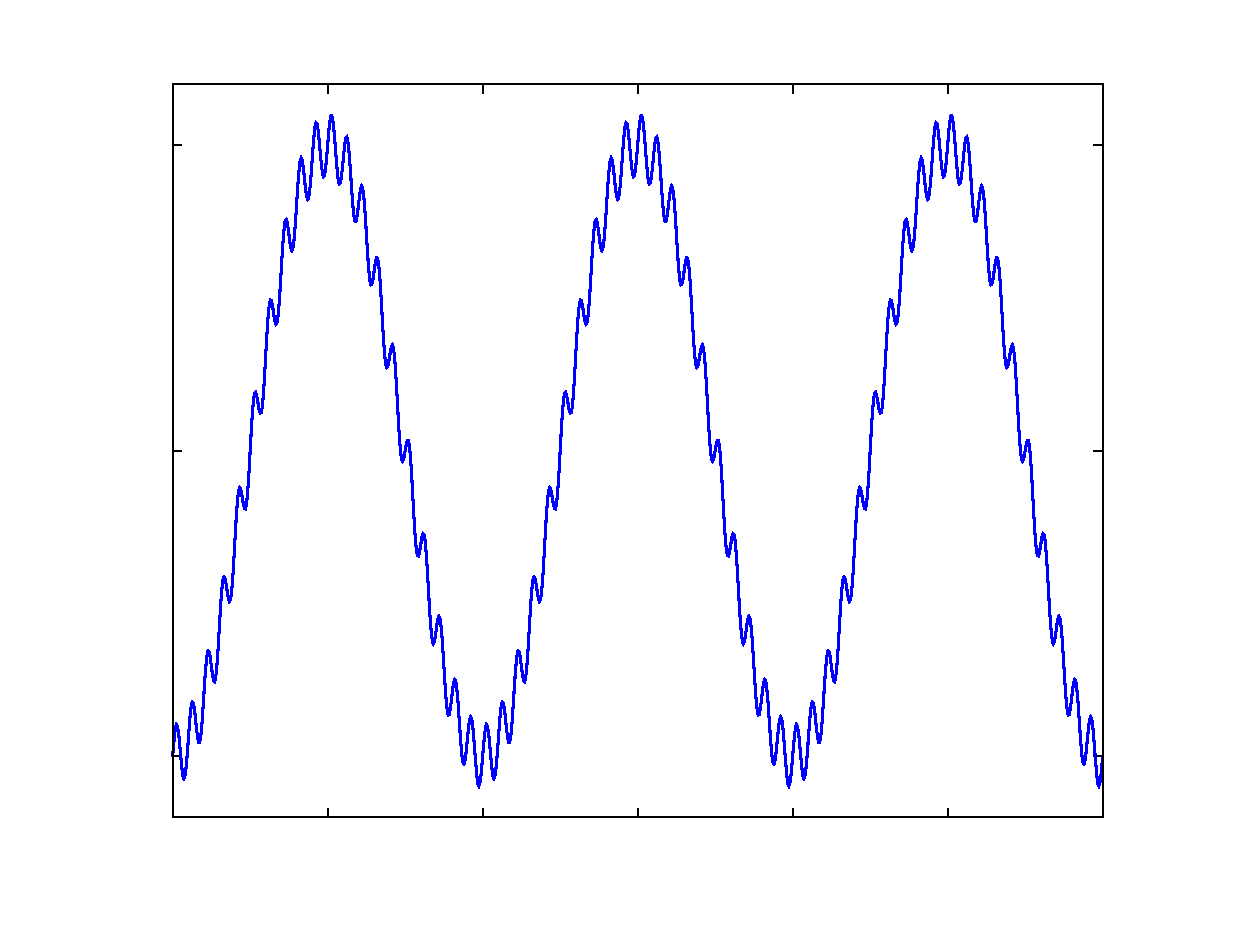
\includegraphics{FuncionEjemplo-inc}
\end{picture}%
\begin{picture}(576,432)(0,0)
\fontsize{30}{0}
\selectfont\put(149.28,42.519){\makebox(0,0)[t]{\textcolor[rgb]{0,0,0}{{-2$\pi$}}}}
\fontsize{30}{0}
\selectfont\put(223.68,34.5){\makebox(0,0)[t]{\textcolor[rgb]{0,0,0}{{-$\pi$}}}}
\fontsize{30}{0}
\selectfont\put(298.08,42.519){\makebox(0,0)[t]{\textcolor[rgb]{0,0,0}{{0}}}}
\fontsize{30}{0}
\selectfont\put(372.48,34.5){\makebox(0,0)[t]{\textcolor[rgb]{0,0,0}{{$\pi$}}}}
\fontsize{30}{0}
\selectfont\put(446.88,42.519){\makebox(0,0)[t]{\textcolor[rgb]{0,0,0}{{2$\pi$}}}}
\fontsize{30}{0}
\selectfont\put(69.8755,76.8599){\makebox(0,0)[r]{\textcolor[rgb]{0,0,0}{{-10}}}}
\fontsize{30}{0}
\selectfont\put(69.8755,223.56){\makebox(0,0)[r]{\textcolor[rgb]{0,0,0}{{0}}}}
\fontsize{30}{0}
\selectfont\put(69.8755,370.26){\makebox(0,0)[r]{\textcolor[rgb]{0,0,0}{{10}}}}
\end{picture}
}
    \vspace{-10pt}
    \caption{Soma de dois harmónicos}
    \label{fig:FuncionEjemplo}
\end{figurebox}
\end{figure}

Poderíamos dizer que $f(x)$ é um sinal com um pequeno nível de ruído. De um ponto de vista prático, é útil poder eliminar o ruído para ficar com a parte de sinal que nos interessa. Uma forma de o fazer seria transformar a função fazendo-a passar por um \textit{filtro} que elimine as frequências não pretendidas.


\subsection{Teorema de Fourier}
No ano de 1807, Joseph Fourier publicou o seu trabalho sobre a propagação do calor. Até então, o problema apenas se sabia resolver quando a fonte de calor se comportava de forma simples (como um harmónico), em cujo caso as soluções se chamavam funções próprias. A ideia de Fourier foi descompor uma excitação qualquer como uma superposição de harmónicos, de modo que a solução é a correspondente superposição de funções próprias.

O teorema que se segue a continuação dá-nos as condições em que é lícito supor que podemos descompor uma função como soma de outras mais simples, harmónicos neste caso.

\begin{mybox}

\textbf{Teorema de Fourier (caso particular).} Seja $f:\mathbb{R}\rightarrow \mathbb{R}$ uma função derivável a pedaços de período $2\pi$. Então existe uma soma de harmónicos que coincide com $f(x)$  naqueles pontos em que $f$ é contínua. Mais explicitamente:

Existem uns únicos coeficientes  $(a_k)$ e $(b_k)$ tais que:
  \begin{equation} \label{eq:RepresentacionFourier}
    f(x) = a_0 + \sum_{k=1}^\infty [a_k\cdot \cos(k\cdot x) + b_k\cdot \sin(k\cdot x)],
  \end{equation}
salvo nos pontos de descontinuidade.
\end{mybox}
Se $x$ é um ponto em que $f$ não é contínua, a equação \eqref{eq:RepresentacionFourier} poderia não ser certa. De facto, neste caso, a soma de harmónicos vale precisamente
\[
\frac{f(x^-) + f(x^+)}{2},
\]
em que $f(x^-)$ e $f(x^+)$ se denotam os limites de $f$ em $x$ pela esquerda e à direita respetivamente.
Por exemplo, podemos considerar o sinal quadrado da Figura \ref{fig:SignalCuadrada}:
\begin{figure}[h]
\begin{figurebox}
    \vspace{5pt}
    \centering
    \scalebox{0.4}{ % Title: glps_renderer figure
% Creator: GL2PS 1.3.8, (C) 1999-2012 C. Geuzaine
% For: Octave
% CreationDate: Thu Jun 26 11:33:43 2014
\setlength{\unitlength}{1pt}
\begin{picture}(0,0)
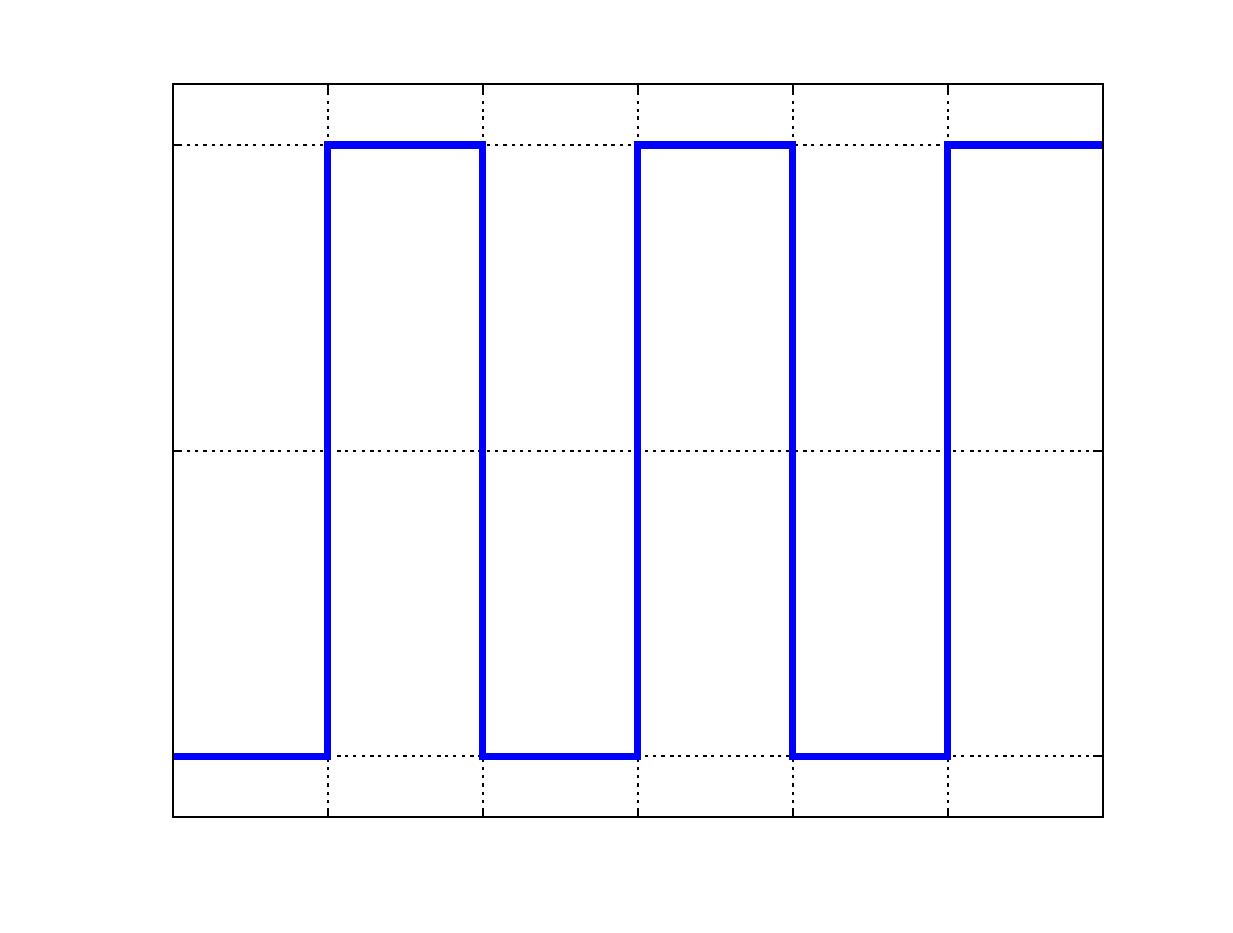
\includegraphics{Cuadrada-inc}
\end{picture}%
\begin{picture}(576,432)(0,0)
\fontsize{30}{0}
\selectfont\put(149.28,42.519){\makebox(0,0)[t]{\textcolor[rgb]{0,0,0}{{-2$\pi$}}}}
\fontsize{30}{0}
\selectfont\put(223.68,34.5){\makebox(0,0)[t]{\textcolor[rgb]{0,0,0}{{-$\pi$}}}}
\fontsize{30}{0}
\selectfont\put(298.08,42.519){\makebox(0,0)[t]{\textcolor[rgb]{0,0,0}{{0}}}}
\fontsize{30}{0}
\selectfont\put(372.48,34.5){\makebox(0,0)[t]{\textcolor[rgb]{0,0,0}{{$\pi$}}}}
\fontsize{30}{0}
\selectfont\put(446.88,42.519){\makebox(0,0)[t]{\textcolor[rgb]{0,0,0}{{2$\pi$}}}}
\fontsize{30}{0}
\selectfont\put(69.8755,76.8599){\makebox(0,0)[r]{\textcolor[rgb]{0,0,0}{{-1}}}}
\fontsize{30}{0}
\selectfont\put(69.8755,223.56){\makebox(0,0)[r]{\textcolor[rgb]{0,0,0}{{0}}}}
\fontsize{30}{0}
\selectfont\put(69.8755,370.26){\makebox(0,0)[r]{\textcolor[rgb]{0,0,0}{{1}}}}
\end{picture}
}
    \vspace{-10pt}
    \caption{Um sinal quadrado}
    \label{fig:SignalCuadrada}
\end{figurebox}
\end{figure}

Este sinal pode ser modelado pela função:
\begin{equation}
  \label{eq:SignalCuadrada}
  f(x) = 
  \begin{cases}
    -1 & \text{si } x\in\left[k\pi,(k+1)\pi\right)\quad\text{para algum }k\in\mathbb{Z}\text{ ímpar}\\
    +1  & \text{si } x\in\left[k\pi,(k+1)\pi\right)\quad\text{para algum }k\in\mathbb{Z}\text{ par}.
  \end{cases}
\end{equation}

É fácil comprovar que esta função tem período $2\pi$. Portanto, o teorema de Fourier \eqref{eq:RepresentacionFourier} permite-nos escrever $f(x)$ como soma de harmónicos. O único problema é saber calcular os coeficientes que aparecem na equação \eqref{eq:RepresentacionFourier}, portanto vamos procurar uma solução.

\subsubsection*{Cálculo dos coeficientes}
Partimos de uma função $f(x)$ com período $2\pi$ que cumpre todos os pré-requisitos do Teorema de representação dado anteriormente. Assim, podemos escrever:
\[
f(x) = a_0 + \sum_{k=1}^\infty a_k\cos(kx) + b_k\sin(kx),
\]
e vamos calcular a seguinte integral:
\begin{align*}
  \int_{-\pi}^{\pi}f(x)\,\mathrm{d}x 
  &=  \int_{-\pi}^{\pi}  \left[a_0 + \sum_{k=1}^\infty a_k\cos(kx) + b_k\sin(kx)\right] \,\mathrm{d}x\\
  &= a_0 \int_{-\pi}^{\pi} \,\mathrm{d}x +  \sum_{k=1}^\infty a_k  \int_{-\pi}^{\pi} \cos(kx) \,\mathrm{d}x + \sum_{k=1}^\infty b_k  \int_{-\pi}^{\pi} \sin(kx) \,\mathrm{d}x\\
  &=  a_0 \cdot 2\pi.
\end{align*}
Em que foi utilizado que
\[
\int_{-\pi}^{\pi} \cos(kx) = 0 = \int_{-\pi}^{\pi} \sin(kx)\qquad \forall k\in \mathbb{N},
\]
para obter
\[
\boxed{a_0 = \frac{1}{2\pi} \int_{-\pi}^{\pi} f(x)\,\mathrm{d}x.}
\]
Com a mesma ideia na mente, podemos fazer outras integrais para deduzir o resto de coeficientes:
\[
\int_{-\pi}^{\pi}f(x) \cdot \cos(kx)\,\mathrm{d}x =\ldots = \pi a_k\qquad\text{e}\qquad  \int_{-\pi}^{\pi}f(x)\cdot  \sin(kx)\,\mathrm{d}x =\ldots = \pi b_k,
\]
donde
\[
\boxed{a_k = \frac{1}{\pi} \int_{-\pi}^{\pi} f(x)\cdot \cos(kx)\,\mathrm{d}x} \qquad \text{e} \qquad  \boxed{b_k = \frac{1}{\pi} \int_{-\pi}^{\pi} f(x)\cdot \sin(kx)\,\mathrm{d}x.}
\]
\qed


Agora que temos uma fórmula para tirar os coeficientes, podemos seguir com o exemplo do sinal quadrado. É um exercício simples demonstrar que neste caso:
\[
a_0 = a_k = 0,\qquad\qquad b_k =
\begin{cases}
  \frac{4}{\pi k}&  \text{se }k\text{ for ímpar}\\
  0              &  \text{se }k\text{ for par. }\\
\end{cases}
\]
De modo que a soma de harmónicos que representa a \eqref{eq:SignalCuadrada} é precisamente:
\begin{equation} \label{eq:Cuadrada}
f(x) = \frac{4}{\pi}\left[\sin x + \frac{1}{3}\sin(3x) + \frac{1}{5}\sin(5x) + \frac{1}{7}\sin(7x) + \frac{1}{9}\sin(9x) + \ldots\right]
\end{equation}


Às vezes é complicado compreender como é que se comporta uma soma infinita. Ainda, na prática apenas podemos somar um número finito de coisas, portanto é necessário comprovar que uma soma finita é uma boa aproximação da função. Esta comparação podemos observá-la na Figura \ref{fig:CuadradaAproximaciones}.

\begin{figure}[h]
\begin{figurebox}
    \vspace{10pt}
    \centering
      \begin{subfigure}{.3\textwidth}
          \centering
          \scalebox{0.25}{ % Title: glps_renderer figure
% Creator: GL2PS 1.3.8, (C) 1999-2012 C. Geuzaine
% For: Octave
% CreationDate: Thu Jun 26 12:41:04 2014
\setlength{\unitlength}{1pt}
\begin{picture}(0,0)
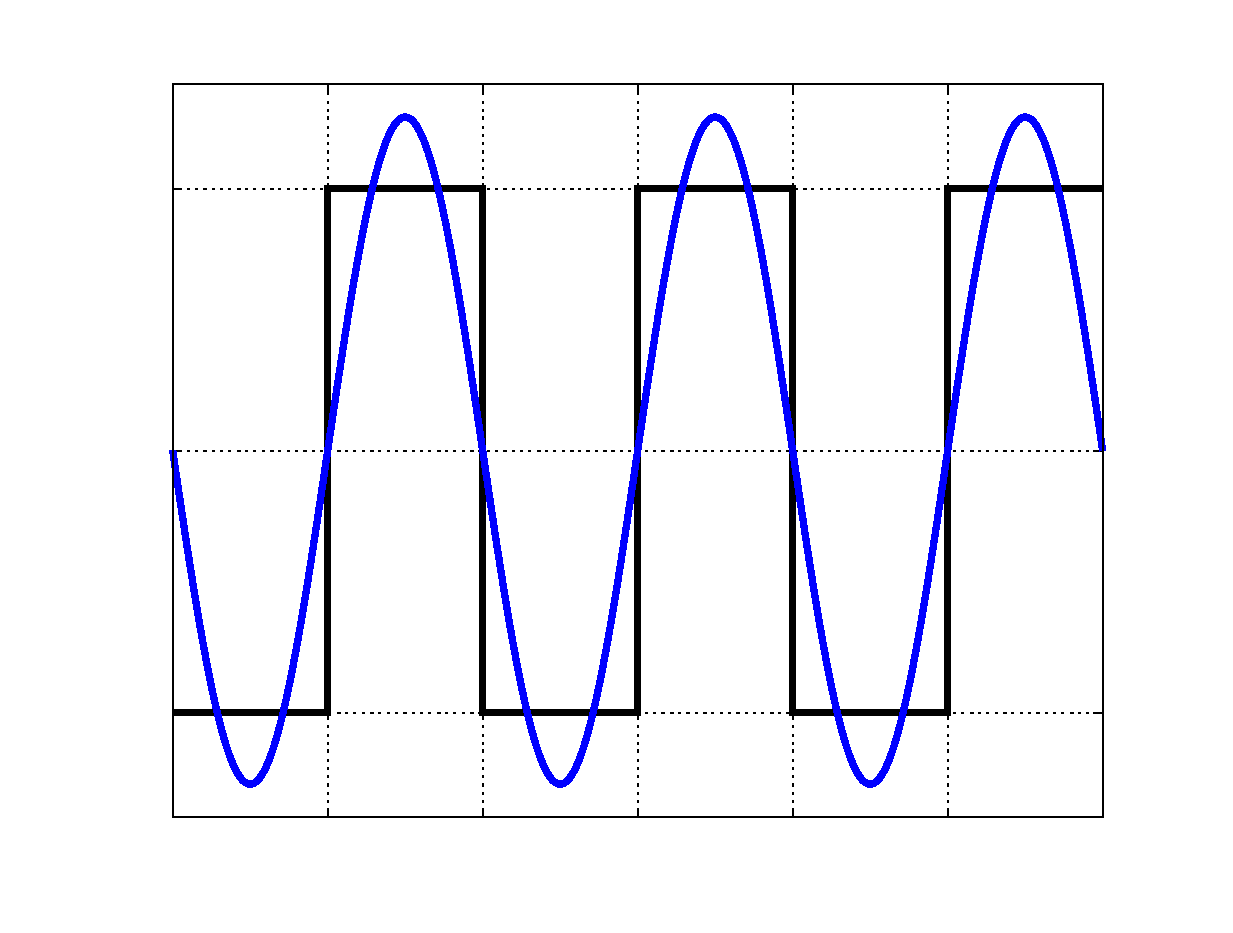
\includegraphics{CuadradaAproximaciones1-inc}
\end{picture}%
\begin{picture}(576,432)(0,0)
\fontsize{30}{0}
\selectfont\put(149.28,42.519){\makebox(0,0)[t]{\textcolor[rgb]{0,0,0}{{-2$\pi$}}}}
\fontsize{30}{0}
\selectfont\put(223.68,34.5){\makebox(0,0)[t]{\textcolor[rgb]{0,0,0}{{-$\pi$}}}}
\fontsize{30}{0}
\selectfont\put(298.08,42.519){\makebox(0,0)[t]{\textcolor[rgb]{0,0,0}{{0}}}}
\fontsize{30}{0}
\selectfont\put(372.48,34.5){\makebox(0,0)[t]{\textcolor[rgb]{0,0,0}{{$\pi$}}}}
\fontsize{30}{0}
\selectfont\put(446.88,42.519){\makebox(0,0)[t]{\textcolor[rgb]{0,0,0}{{2$\pi$}}}}
\fontsize{30}{0}
\selectfont\put(69.8755,97.8169){\makebox(0,0)[r]{\textcolor[rgb]{0,0,0}{{-1}}}}
\fontsize{30}{0}
\selectfont\put(69.8755,223.56){\makebox(0,0)[r]{\textcolor[rgb]{0,0,0}{{0}}}}
\fontsize{30}{0}
\selectfont\put(69.8755,349.303){\makebox(0,0)[r]{\textcolor[rgb]{0,0,0}{{1}}}}
\end{picture}
}
          \caption{1 harmónico}
          \label{fig:0a} 
      \end{subfigure} %
      \begin{subfigure}{.3\textwidth}
          \centering
          \scalebox{0.25}{% Title: glps_renderer figure
% Creator: GL2PS 1.3.8, (C) 1999-2012 C. Geuzaine
% For: Octave
% CreationDate: Thu Jun 26 12:41:07 2014
\setlength{\unitlength}{1pt}
\begin{picture}(0,0)
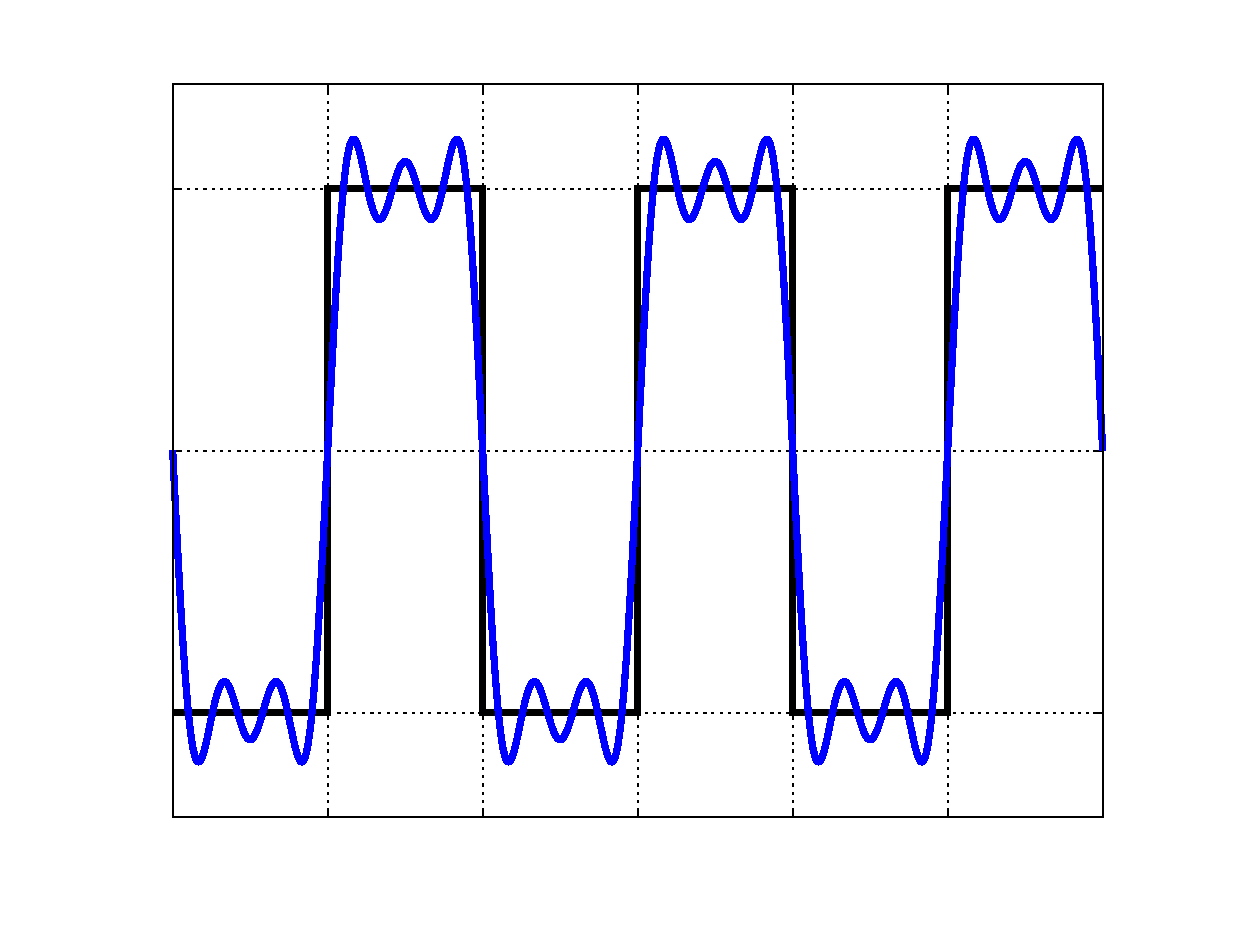
\includegraphics{CuadradaAproximaciones3-inc}
\end{picture}%
\begin{picture}(576,432)(0,0)
\fontsize{30}{0}
\selectfont\put(149.28,42.519){\makebox(0,0)[t]{\textcolor[rgb]{0,0,0}{{-2$\pi$}}}}
\fontsize{30}{0}
\selectfont\put(223.68,34.5){\makebox(0,0)[t]{\textcolor[rgb]{0,0,0}{{-$\pi$}}}}
\fontsize{30}{0}
\selectfont\put(298.08,42.519){\makebox(0,0)[t]{\textcolor[rgb]{0,0,0}{{0}}}}
\fontsize{30}{0}
\selectfont\put(372.48,34.5){\makebox(0,0)[t]{\textcolor[rgb]{0,0,0}{{$\pi$}}}}
\fontsize{30}{0}
\selectfont\put(446.88,42.519){\makebox(0,0)[t]{\textcolor[rgb]{0,0,0}{{2$\pi$}}}}
\fontsize{30}{0}
\selectfont\put(69.8755,97.8169){\makebox(0,0)[r]{\textcolor[rgb]{0,0,0}{{-1}}}}
\fontsize{30}{0}
\selectfont\put(69.8755,223.56){\makebox(0,0)[r]{\textcolor[rgb]{0,0,0}{{0}}}}
\fontsize{30}{0}
\selectfont\put(69.8755,349.303){\makebox(0,0)[r]{\textcolor[rgb]{0,0,0}{{1}}}}
\end{picture}
}
          \caption{3 harmónicos}
          \label{fig:0b}
      \end{subfigure} %
      \begin{subfigure}{.3\textwidth}
          \centering
          \scalebox{0.25}{% Title: glps_renderer figure
% Creator: GL2PS 1.3.8, (C) 1999-2012 C. Geuzaine
% For: Octave
% CreationDate: Thu Jun 26 12:41:11 2014
\setlength{\unitlength}{1pt}
\begin{picture}(0,0)
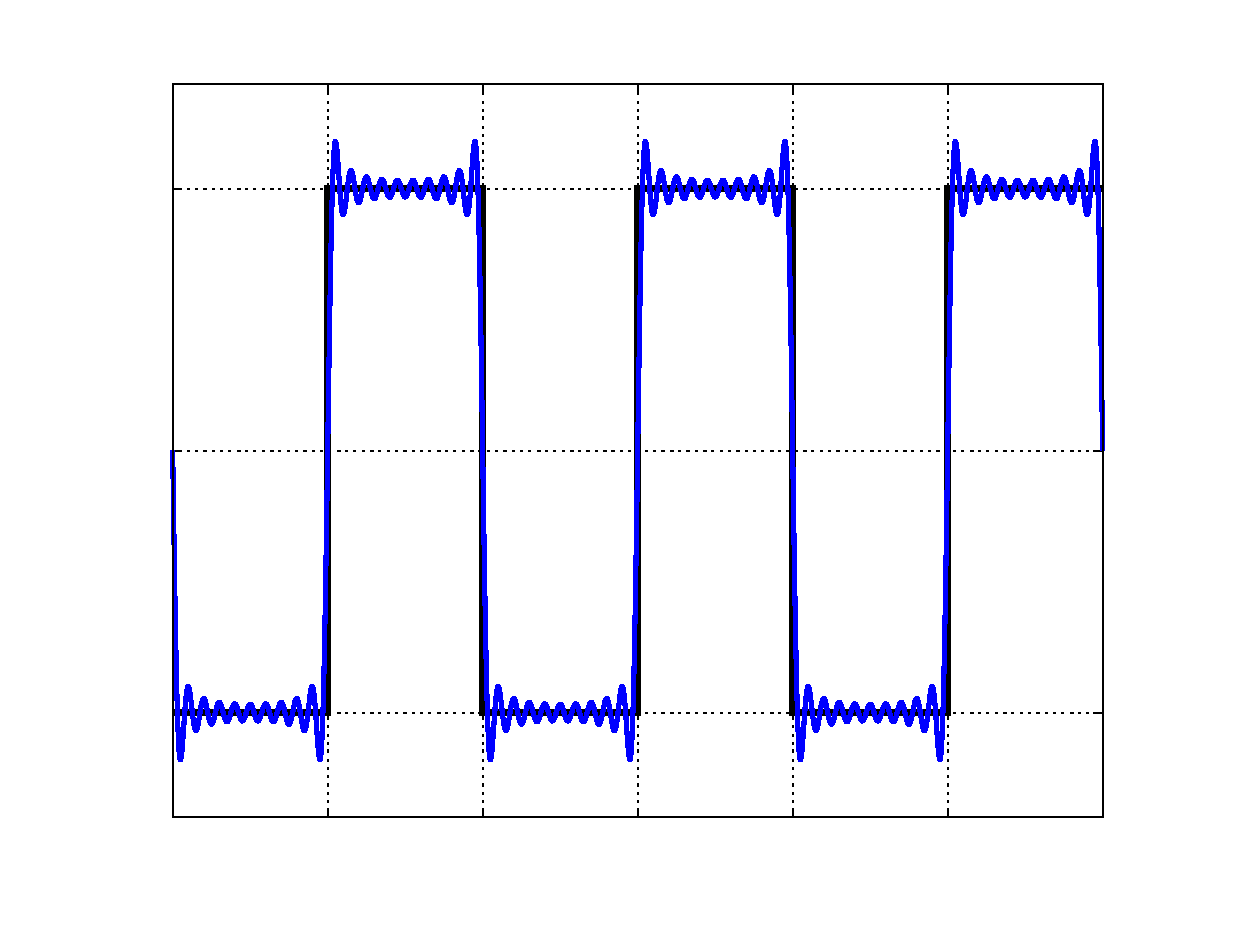
\includegraphics{CuadradaAproximaciones10-inc}
\end{picture}%
\begin{picture}(576,432)(0,0)
\fontsize{30}{0}
\selectfont\put(149.28,42.519){\makebox(0,0)[t]{\textcolor[rgb]{0,0,0}{{-2$\pi$}}}}
\fontsize{30}{0}
\selectfont\put(223.68,34.5){\makebox(0,0)[t]{\textcolor[rgb]{0,0,0}{{-$\pi$}}}}
\fontsize{30}{0}
\selectfont\put(298.08,42.519){\makebox(0,0)[t]{\textcolor[rgb]{0,0,0}{{0}}}}
\fontsize{30}{0}
\selectfont\put(372.48,34.5){\makebox(0,0)[t]{\textcolor[rgb]{0,0,0}{{$\pi$}}}}
\fontsize{30}{0}
\selectfont\put(446.88,42.519){\makebox(0,0)[t]{\textcolor[rgb]{0,0,0}{{2$\pi$}}}}
\fontsize{30}{0}
\selectfont\put(69.8755,97.8169){\makebox(0,0)[r]{\textcolor[rgb]{0,0,0}{{-1}}}}
\fontsize{30}{0}
\selectfont\put(69.8755,223.56){\makebox(0,0)[r]{\textcolor[rgb]{0,0,0}{{0}}}}
\fontsize{30}{0}
\selectfont\put(69.8755,349.303){\makebox(0,0)[r]{\textcolor[rgb]{0,0,0}{{1}}}}
\end{picture}
}
          \caption{10 harmónicos}
          \label{fig:0c}
      \end{subfigure}
      % 
      \caption{Aproximação por harmónicos de um sinal quadrado.}
      \label{fig:CuadradaAproximaciones}
    
\end{figurebox}
\end{figure}



Tudo o anterior pode ser generalizado a funções de período $2T$ em vez de $2\pi$, só que nesse caso vamos ter que esticar ou encolher os harmónicos para que tenham esse mesmo período. 


\begin{mybox}

\textbf{Teorema de Fourier.} Seja $f:\mathbb{R}\rightarrow \mathbb{R}$ uma função derivável a pedaços de período $2T$. Então existe uma soma de harmónicos que coincide com $f(x)$ naqueles pontos em que $f$ é contínua. Mais explicitamente:

Existem uns únicos coeficientes  $(a_k)$ e $(b_k)$ tais que:
  \begin{equation} \label{eq:RepresentacionFourier2}
    f(x) = a_0 + \sum_{k=1}^\infty a_k\cos(\omega_kx) + b_k\sin(\omega_kx)\quad \text{ sendo }\quad \omega_k = \frac{k \pi}{T},
  \end{equation}
salvo nos pontos de descontinuidade.
\end{mybox}

O cálculo dos coeficientes muda um pouco, mas qualitativamente a situação é a mesma. Um desenvolvimento mais detalhado pode-se encontrar em  \cite{Asmar}.



\subsection{Uma aplicação rápida}
Como já foi mencionado, a Figura \ref{fig:CuadradaAproximaciones} mostra que a aproximação se aproxima rápido à função\footnote{Salvo pelas oscilações que se produzem nos pontos de descontinuidade, o que é conhecido como \textit{fenómeno de Gibbs}.}. Vamos pensar um bocado como aproveitar isso.

\subsubsection*{O problema de guardar uma função}
Vamos supor que queremos guardar uma canção num arquivo. O som gravado pode ser representado por um sinal, que não deixa de ser uma função que chamaremos $f(t)$. Uma solução simples seria guardar muitíssimos pares da forma $(t, f(t))$. De facto, deveríamos guardar infinitos pares desta forma para conhecer a função na sua totalidade. Ora bem, como podem imaginar, guardar infinitos valores não parece muito eficiente.

O que é que acontece se encontramos o desenvolvimento de Fourier? A situação não parece mudar muito, uma vez que um conhecimento completo da função nos exigiria guardar os infinitos pares de coeficientes $(a_k, b_k)$. No entanto, a situação sim mudou radicalmente. Agora podemos decidir que vamos ficar (por exemplo) com os 100 primeiros pares de coeficientes, isso é muito mais acessível.

Evidentemente, a função que reconstruamos a partir destes coeficientes não vai ser igual, dado que não temos toda a informação, mas se a série de Fourier converger rapidamente, deveria ser enormemente parecida com a original. Por outras palavras, o nosso ouvido não será capaz de distinguir a diferença, e ao mesmo tempo estaremos a poupar muitíssimo espaço. Em ideias semelhantes são baseados os algoritmos de compressão de arquivos que se utilizam nos computadores, como o mp3.

\begin{mybox}
  Para acabar, vamos ver uma das pequenas maravilhas que aparecem quando estudamos as séries de Fourier. Se avaliarmos em $x=\frac{\pi}{2}$ na equação \eqref{eq:Cuadrada} e despejarmos, encontramos a bonita identidade:
  \[
    \frac{\pi}{4} = 1 - \frac{1}{3} + \frac{1}{5} - \frac{1}{7} + \ldots .
  \]
\end{mybox}

\section{Enfoque complexo}\label{s:s3}
Até agora temos trabalhado com números reais, combinando engenhosamente senos e cossenos para chegar ao resultado pretendido. No entanto, resulta que os números complexos possuem certas peculiaridades que facilitam todos os cálculos descritos até agora.

\subsection{Números complexos}
Fazemos um breve resumo (para ampliar, consultar \cite{Agarwal}). Recordemos que é comum expressar um número complexo $z\in\mathbb{C}$ em forma binómica, isto é:
\[
z = a + ib,
\]
em que $i$ se conhece como unidade imaginária (que satisfaz $i^2=-1$), no entanto $a$ e $b$ são números reais que recebem o nome de parte real e imaginária de $z$ respetivamente, isso escreve-se habitualmente como:
\[
\operatorname{Re} (z) = a, \qquad \operatorname{Im} (z) = b.
\]
Um conceito que aparece com frequência é o conjugado de um número complexo $z=a+ib\in\mathbb{C}$, que se denota habitualmente como $\overline{z}\in \mathbb{C}$, e é definido por
\begin{equation}
  \label{eq:Conjugado}
  \overline{z} = a - ib.
\end{equation}
O seguinte que vamos revisar será o análogo complexo da função exponencial.

\subsection{Exponencial complexa}
A forma mais rápida de construir este conceito é recorrer às séries de potências. Numa clara analogia com a exponencial real, podemos apresentar a exponencial complexa como a função $\text{exp}:\mathbb{C}\longrightarrow \mathbb{C}$ definida por:
\begin{equation}
  \label{eq:DefinicionExponencial}
  \text{exp}(z) = 1 + z + \frac{z^2}{2!} + \frac{z^3}{3!} + \ldots = \sum_{n=0}^\infty \frac{z^n}{n!}.
\end{equation}

Na prática, é comum escrever simplesmente $e^z$ em vez de $\text{exp}(z)$. Esta função tem muitíssimas propriedades interessantes. Nós, por enquanto, vamos destacar que para qualquer par de números complexos $z,w\in\mathbb{C}$ temos:
\begin{equation}
  \label{eq:PropiedadExponencial}
  e^{z+w} = e^z e^w,
\end{equation}
bem como
\begin{equation}
  \label{eq:ConjugadoExponencial}
  e^{\overline{z}} = \overline{e^z}.
\end{equation}
Em particular, se considerarmos um número complexo na sua forma binómica podemos utilizar \eqref{eq:PropiedadExponencial}:
\[
e^z = e^{a+ib} = e^a e^{ib},
\]
e agora pode estudar-se o desenvolvimento em série de potências \eqref{eq:DefinicionExponencial} da exponencial que envolve a parte imaginária para demonstrar finalmente:
\[
e^{a+ib} = e^a \left[\cos b + i\sin b\right].
\]
Aqui deveríamos começar a ver o potencial do que estamos a fazer. Começámos a trabalhar com números complexos, e resulta que ao fazer exponenciais encontramos senos e cossenos. Isso significa que podemos aproveitar todo o nosso conhecimento sobre exponenciais e utilizá-lo na altura de trabalhar com harmónicos.

\begin{mybox}
Como apontamento histórico, se considerarmos um número que apenas tem parte imaginária encontramos a bonita igualdade
\begin{equation}
  \label{eq:EulerFormula}
  e^{i\theta}\ = \cos\theta + i\sin\theta,
\end{equation}
conhecida como \textbf{fórmula de Euler}, que no caso particular $\theta = \pi $  nos leva à famosa \textbf{identidade de Euler}
\[e^{i\pi} + 1 = 0.\]
\end{mybox}


\subsection{Aplicação às séries de Fourier}
Como já dissemos, utilizaremos as exponenciais complexas para expressar as somas de harmónicos, para o que convém recordar todas as relações entre estes dois conceitos. Por um lado temos a fórmula de Euler \eqref{eq:EulerFormula} e por outro:
\begin{equation}
  \label{eq:ArmonicosDesdeExponencial}
  \cos x = \frac{e^{ix} + e^{-ix}}{2}, \qquad \sin x = \frac{e^{ix} - e^{-ix}}{2i}.
\end{equation}
Portanto, vamos considerar uma função $f:\mathbb{R}\longrightarrow\mathbb{R}$ de período $2\pi$ a que aplicar o teorema de Fourier. Se agora substituirmos \eqref{eq:ArmonicosDesdeExponencial} no $k$-éssimo termo do desenvolvimento descrito em \eqref{eq:RepresentacionFourier} encontramos:
\[
a_k\cos(kx) + b_k\sin(kx) = a_k \frac{e^{ikx} + e^{-ikx}}{2} + b_k \frac{e^{ikx} - e^{-ikx}}{2i} = \frac{1}{2}(a_k-ib_k) e^{ikx} + \frac{1}{2}(a_k+ib_k) e^{-ikx}.
\]
E portanto, passámos de uma combinação de harmónicos para uma combinação de exponenciais, que podemos reescrever como:
\begin{equation}
  \label{eq:kesimoExponenciales}
  a_k\cos(kx) + b_k\sin(kx) = c_k\ e^{ikx} + c_{-k}\ e^{-ikx} \qquad \text{com}\quad c_{\pm k} = \frac{1}{2}(a_k \mp ib_k).
\end{equation}
Para ganhar generalidade, claramente devemos definir $c_0=a_0$ e por fim podemos dar uma formulação alternativa do desenvolvimento de Fourier \eqref{eq:RepresentacionFourier}:
\begin{equation}
  \label{eq:FourierComplejo}
  f(x) = \sum_{k=-\infty}^\infty c_k e^{ikx}.
\end{equation}
Para terminar de arredondar o resultado, vamos dar uma vista de olhos aos coeficientes. Estaria muito bem poder ter uma fórmula que não nos obrigue a calcular primeiro os coeficientes reais e depois os complexos, e com efeito, basta comprovar que
\[\boxed{
c_k = \frac{1}{2\pi} \int _{-\pi}^\pi f(x) e^{-ikx} \,\text{d}x
}\]
nos leva diretamente aos coeficientes complexos\footnote{Para isso haveria que definir cuidadosamente como integrar funções complexas, mas é suficiente que separemos a parte real e imaginária usando \eqref{eq:EulerFormula} e integremos cada uma por separado, sendo assim o resultado imediato.}.

No caso em que as funções tenham período $2T$, temos um resultado similar, mas de novo mudam levemente as fórmulas para calcular os coeficientes. A formulação alternativa do teorema de Fourier neste caso é:

\begin{mybox}

\textbf{Teorema de Fourier (formulação complexa).} Seja $f:\mathbb{R}\rightarrow \mathbb{R}$ uma função derivável a pedaços de período $2T$. Então existe uma soma de harmónicos que coincide com $f(x)$ naqueles pontos em que $f$ é contínua. Mais explicitamente:

Existem uns únicos coeficientes  $(c_k)$ tais que:
  \begin{equation} \label{eq:RepresentacionFourier3}
    f(x) = \sum_{k=-\infty}^\infty c_ke^{i\omega_k x}\quad \text{ sendo }\quad \omega_k = \frac{k \pi}{T},
  \end{equation}
salvo nos pontos de descontinuidade.
\end{mybox}

\begin{mybox}
\begin{mybox}
Criamos uma aplicação web , onde você pode entender geometricamente os conceitos neste artigo . O link é:

\url{http://fourieranalysis.github.io/series.html}.
\end{mybox}
\end{mybox}
\bibliographystyle{plain}
\bibliography{fourier1}

\newpage

%%% Local Variables: 
%%% mode: latex
%%% TeX-master: "matematicaseningenieria"
%%% End: 


